\chapter*{ВВЕДЕНИЕ}
\addcontentsline{toc}{chapter}{ВВЕДЕНИЕ}
Сжатие данных - это процесс уменьшения размера данных с целью уменьшения объема памяти, занимаемого этими данными, или увеличения скорости передачи данных. Существуют различные методы сжатия данных, такие как алгоритмы с потерями и без потерь, которые позволяют сжимать различные типы данных, включая текст, изображения, аудио и видео.

Цель данной работы~---~разработка алгоритма сжатия информации.

Для достижения поставленной цели необходимо выполнить следующие задачи.

\begin{enumerate}[label=\arabic*)]
	\item Изучить алгоритм LZW.
	\item Спроектировать алгоритм LZW.
	\item Реализовать алгоритм LZW.
	\item Протестировать реализацию алгоритма.
\end{enumerate}

\chapter{Теоретический раздел}

\section{LZW}

Алгоритм LZW (Lempel-Ziv-Welch) - это универсальный алгоритм сжатия данных, который был разработан в 1984 году. Он широко используется для сжатия текстовых данных и изображений.

Принцип работы алгоритма LZW заключается в замене повторяющихся последовательностей символов на коды, что позволяет сократить объем данных. Алгоритм основан на словаре, который содержит все возможные комбинации символов, которые могут встретиться в исходных данных.

\textbf{Шаги алгоритма LZW:}

1. Инициализация словаря: в начале работы алгоритма создается словарь, который содержит все возможные символы (например, буквы алфавита) и коды для них.

2. Чтение исходных данных: алгоритм читает исходные данные и ищет самую длинную подстроку, которая уже есть в словаре.

3. Добавление новой последовательности в словарь: если найденная подстрока отсутствует в словаре, то она добавляется в словарь с новым кодом.

4. Замена последовательности на код: найденная подстрока заменяется на соответствующий ей код из словаря.

5. Повторение шагов 2-4: процесс поиска повторяющихся последовательностей и их замены на коды продолжается до тех пор, пока все исходные данные не будут обработаны.

6. Вывод закодированных данных: после завершения работы алгоритма получается закодированный поток данных, который занимает меньше места, чем исходные данные.

Алгоритм LZW имеет ряд преимуществ, таких как высокая степень сжатия, относительно простая реализация и возможность адаптации к различным типам данных. Однако он также имеет некоторые ограничения, например, он может потребовать больше памяти для хранения словаря при работе с большими данными.

\chapter{Конструкторский раздел}

\section{Разработка алгоритма}

На рисунках \ref{img:lzw} и \ref{img:dec} представлены схемы реализации сжатия и разжатия данных алгоритмом LZW соответственно.

\begin{table}[H]
	\centering
	\begin{tabular}{p{1\linewidth}}
		\centering
		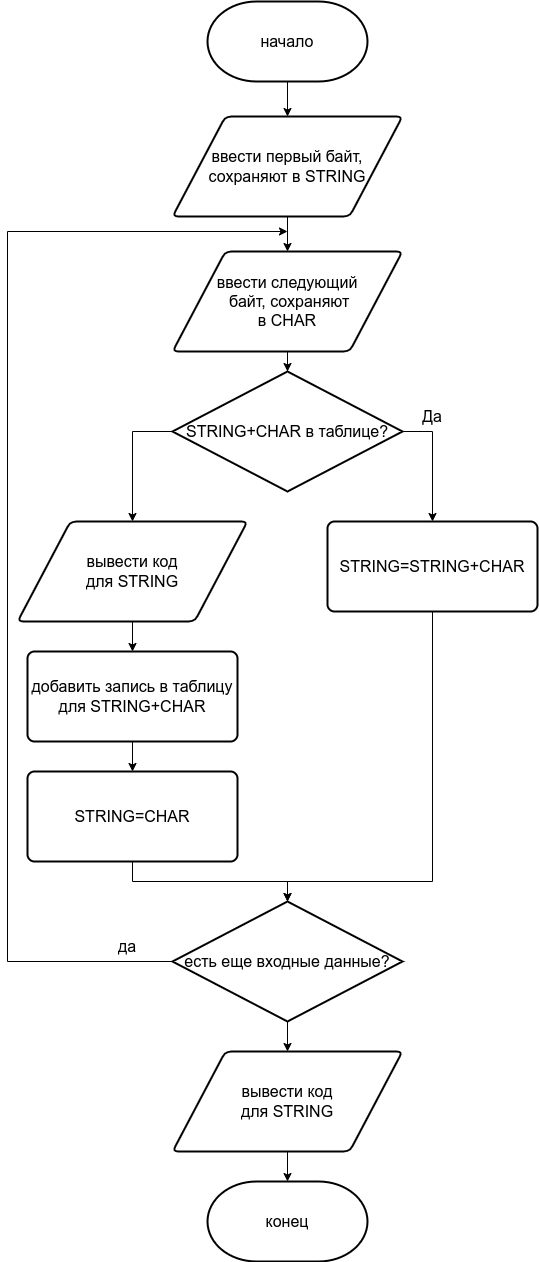
\includegraphics[width=0.4\linewidth]{assets/lzw.png}
		\captionof{figure}{Схемы для реализации сжатия данных алгоритмом LZW}
		\label{img:lzw}
	\end{tabular}
\end{table}

\begin{table}[H]
	\centering
	\begin{tabular}{p{0.7\linewidth}}
		\centering
		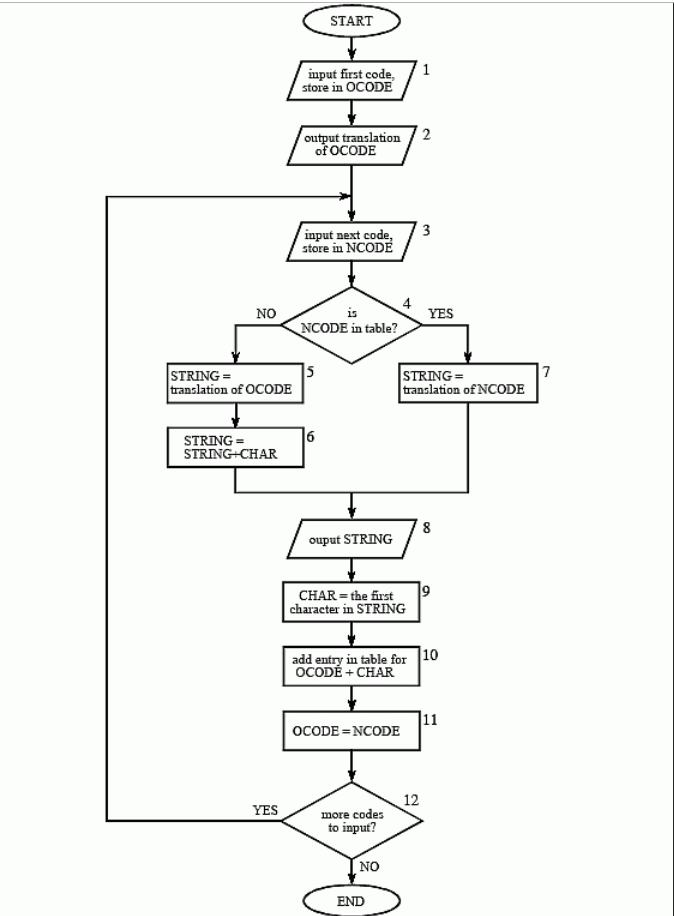
\includegraphics[width=1\linewidth]{assets/dec.png}
		\captionof{figure}{Схемы для реализации разжатия данных алгоритмом LZW}
		\label{img:dec}
	\end{tabular}
\end{table}